\documentclass[a4paper, 11pt, titlepage]{article}
\usepackage{fancyhdr}
\usepackage{graphicx}
\usepackage{imakeidx}
\usepackage{makeidx}
\usepackage{mathtools}
\usepackage[spanish]{babel}
\usepackage{eurosym}
\usepackage{hyperref}
\usepackage{amssymb}
\usepackage{listings}
\usepackage{xcolor}

% \setcounter{secnumdepth}{5}
% \setcounter{tocdepth}{5}

\title{Sistemas expertos en combinación con lógica difusa}
\author{Francisco Javier Balón Aguilar}

\begin{document}

\maketitle
\renewcommand{\contentsname}{Índice}
\tableofcontents
\newpage

\section*{Prólogo}

\section{Introducción}\label{introduccion}

    Generalmente, se considera a alguien un experto en un problema cuando éste tiene
    conocimiento especializado sobre dicho problema, o en otras palabras, tiene dominio 
    sobre éste.  También en el área de la inteligencia artificial se conoce como 
    sistemas expertos a aquellos con conocimiento especializado sobre dicho problema, así 
    como conocimiento sobre el dominio.

    Los sistemas expertos buscan la emulación o imitación del razonamiento humano, 
    restringiéndose a un espacio de conocimiento limitado, razonando como lo harían
    --siguiendo una serie de pasos pertinentes-- un experto humano de diversas materias 
    o disciplinas, como médico, analista, empresario, etc. Su uso será rápidamente en el 
    futuro debido principalmente a su uso en industria y medicina, principalmente.

    La lógica difusa proporciona una serie de mecanismos de inferencia que permite simular 
    procesos de razonamiento humano, al igual que un sistema experto (lo que permite su 
    fácil adopción y aplicación en éste). La lógica difusa proporciona un marco matemático 
    que permite modelar la incertidumbre de los procesos cognitivos [evidentemente humanos]
    de forma que puedan ser computazionables.

\section{Sistemas expertos}

    Como ya hemos adelantado en la introducción (véase sección \ref{introduccion}), un sistema 
    experto es un software que imita el comportamiento de un experto en la solución de un problema, 
    generalmente en un campo o disciplina concreta, aplicando deducción lógica y una serie de 
    pasos en la solución de éste.

    Un sistema experto trae consigo determinadas limitaciones a tener en cuenta:
    
    \begin{itemize}
        \item El conocimiento en sí es difícil de extraer y normalizar de los expertos.
        \item La aproximación de cada experto a un determinado problema evaluado puede ser diferente.
        \item Tienen una noción limitada a su campo y acerca del contexto del problema.
    \end{itemize}

    Aun así presentando una serie de ventajas con respecto a los sistemas tradicionales de 
    resolución de problemas basados en algoritmos:

    \begin{itemize}
        \item Presentan capacidad de toma de decisiones.
        \item Calculan resultados, basados en heurísticas.
        \item Ofrecen explicaciones de sus resultados.
        \item Usan reglas de inferencia.
        \item Proporcionan bases de conocimiento (deductivo).
        \item Manejan conocimiento impreciso, contradictorio e incompleto.
        \item Usan datos y lenguajes simbólicos.
    \end{itemize}

    \subsection{Arquitectura de un sistema experto}

        \begin{figure}[htp]
            \centering
            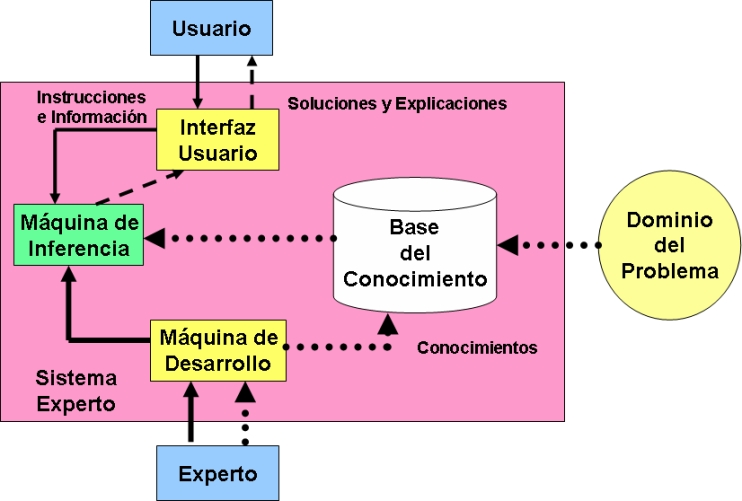
\includegraphics[width=0.7\textwidth]{resources/sistemaexperto.jpg}
            \caption{Arquitectura de un sistema experto.}
            \label{sistemaexperto}
        \end{figure}

        Un sistema experto se compone de los siguientes elementos constituyentes:

        \begin{itemize}
            \item \textbf{Base de conocimiento}. Contiene el conocimiento sobre el 
            dominio, que se obtiene del conocimiento del experto y se codifican en ésta.
            La forma más clásica de representación del conocimiento son las reglas\footnote{
                Una regla es una estructura condicional que relaciona lógicamente la 
                información contenida en parte del antecedente con otra información 
                contenida en la parte del consecuente.
            }.
            \item \textbf{Base de hechos} o memoria de trabajo. Contiene los hechos sobre 
            un problema ya descubierto previamente, que se introduce en la base de hechos 
            durante una consulta con el sistema experto. El sistema empareja esta información  
            con el conocimiento disponible en la base de conocimientos para deducir nuevos 
            hechos.
            \item \textbf{Motor de inferencia}. El razonamiento humano es modelado como proceso 
            con un módulo como el motor de inferencia, que trabaja con la información contenida 
            en la base de hechos para deducir nuevos hechos y contrastando hechos particulares 
            de la base de conocimientos para obtener conclusiones acerca del problema.
            \item \textbf{Interfaz de usuario}. La interfaz que comunica al software con el usuario, 
            generalmente en lenguaje natural, buscando ser interactiva e imitando la conversación
            entre humanos.
        \end{itemize}


\section{Lógica difusa}

    Como ya hemos adelantado en la introducción (véase sección \ref{introduccion}), la lógica difusa, 
    también conocida como lógica borrosa, se basa en lo relativo de lo observado como posición 
    diferencial. Toma dos valores aleatorios, pero contextualizados y referidos entre sí.

    Trae una serie de ventajas tales como:

    \begin{itemize}
        \item Facilidad de implementación.
        \item Buenos resultados contrastables, en procesos no lineales y de difícil modelación.
        \item Modo de comportamiento similar al comportamiento humano.
        \item Velocidad en la resolución de problemas.
        \item Abstracción del modelo matemático.
    \end{itemize}

    Que, sin embargo, contrasta con una serie de desventajas a tener en cuenta:

    \begin{itemize}
        \item Múltiples definiciones de operadores y reglas de inferencia difusas.
        \item Dificultad de interpretación de valores difusos, es decir, una semántica no clara.
        \item No hay una buena justificación operadores difusos.
        \item Requiere de tiempo y datos previos al aprendizaje.
    \end{itemize}

    \subsection{Arquitectura de un sistema de lógica difusa}

        \begin{figure}[htp]
            \centering
            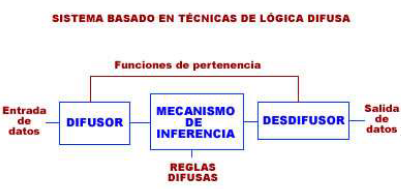
\includegraphics[width=0.7\textwidth]{resources/logicadifusa.png}
            \caption{Arquitectura de un sistema basado en lógica difusa.}
            \label{logicadifusa}
        \end{figure}

        Un sistema basado en lógica difusa se compone de los siguientes elementos constitutivos:

        \begin{itemize}
            \item \textbf{Difusor}. El ingreso del bloque difusor está constituido por los 
            datos de las variables de interés para el estudio. El proceso, conformado por 
            los grados de pertenencia de estas variables de entrada, implica conocer y/o 
            asumir las respectivas funciones de pertenencia.
            \item \textbf{Motor de inferencia}. Inferir consiste en obtener una conclusión 
            o deducir algo de otra cosa, estando relacionado con la implicación, entendida como 
            repercusión o consecuencia. En términos proposicionales se escribe para para indicar 
            que el cumplimiento de una proposición tiene como consecuencia el cumplimiento de otra.
            Se expresa como el condicional \textit{if} (si... entonces...).
            \item \textbf{Desfusificador}. La salida del bloque de inferencia continúa siendo difuso,
            pero ya relacionado con la variable de entrada. Debe expresarse en resultados concretos.
        \end{itemize}

    \subsection{Funcionamiento matemático/técnico de la lógica difusa}

        La lógica difusa define el grado de pertenencia que tiene un 
        objeto a una clase particular. Este grado de pertenencia es un valor entre cero y uno que 
        indica la adherencia de un grupo a otro\footnote{
            Zadeh, 1965
        }. Los conjuntos difusos son una extensión 
        de los conjuntos clásicos, donde se añade una función de pertenencia, es decir, que a cada 
        elemento del universo se le asocia un grado de pertenencia, definido como un número real entre 
        0 y 1\footnote{
            Johansson,1993
        }. Mientras el grado de pertenencia sea más cercano a 1, significa que el 
        elemento pertenece en un mayor grado a dicho conjunto. Caso contrario ocurre si el valor se 
        acerca a 0. Así es, cómo se introduce el concepto de conjunto o subconjunto difuso y se lo 
        asocia a un determinado valor lingüístico, definido por una palabra o etiqueta lingüística, 
        donde está el nombre del conjunto o subconjunto. 
        
        Por cada conjunto se define una función de 
        pertenencia o membresía denominada $\mu A(x)$, que indica el grado en que la variable x está incluida 
        en el concepto representado por la etiqueta $A (0 \leq \mu A(x) \leq 1)$. 

        El concepto de lógica difusa define la base de reglas como la manera que tiene un sistema difuso 
        de guardar el conocimiento lingüístico, el cual le permite resolver el problema para el cual ha 
        sido diseñado. Estas reglas son del tipo “Si-Entonces” y asocian uno o más conjuntos difusos de 
        entrada llamados antecedentes con un conjunto difuso de salida llamado consecuente. Para el caso 
        del modelo propuesto, se asocian los conjuntos de entrada con el operador lógico \textit{AND} para tener 
        un conjunto de salida o consecuente\footnote{
            De Negri y De vito, 2006
        }.

        Una vez establecida la base de reglas para cada una de las fases del sistema experto difuso, 
        es necesario, como ya vimos anteriormente en la arquitectura de ésta, definir el método de 
        inferencia y agregación que determinan la salida o respuesta del sistema. Mediante el proceso de 
        inferencia, se obtiene el conjunto difuso de salida. Este conjunto es calculado de acuerdo a las
        reglas establecidas y al método de inferencia utilizado. Generalmente, se emplea el método de 
        inferencia por mínimos (Min) de Mamdami definido según la ecuación\footnote{
            Zadeh, 1965
        }:

        \[
            min(\mu, \mu_w(z)) \forall z    
        \]

        Donde $\mu_w$ es la función de pertenencia del conjunto de salida $w$.

        El método de agregado agrupa todos los conjuntos de salida, de cada una de las reglas establecidas, 
        para obtener un único conjunto difuso. Para el modelo experto difuso propuesto, se utiliza el método 
        de agregación por máximos (Max), descrito por la ecuación:
        
        \[
            C' = [(z, \mu_C' (z) / z \in Z)]    
        \]

        Que agrupa los máximos valores, de cada regla asignada, que han sido obtenidos mediante el proceso 
        de inferencia difuso. Y donde $Z$ es igual al universo del discurso de la variable de salida y:
        
        \[
            \mu_C' (z) = Max(C1', C2',... Cn')    
        \]

        Finalmente, el proceso de defusificación consiste en un proceso matemático usado para convertir 
        un conjunto difuso en un número real\footnote{
            Llano et. al., 2007
        }. El conjunto que se ha obtenido del proceso de inferencia y agregación, debe ser transformado 
        en un valor numérico que pueda ser interpretado por elementos externos. Con el fin de determinar 
        qué método de defusificación se emplearía en el modelo, se realizó un análisis previo, utilizando
        un conjunto menor de datos. El resultado de este análisis arrojó que el método del centroide de 
        área posee un error porcentual más bajo.

        En este método, el centro de gravedad es aproximado por el centro de gravedad de un arreglo de 
        masas puntuales, las cuales son el centro de gravedad de cada conjunto de salida correspondiente 
        a cada regla, con masa igual al grado de pertenencia en ese punto de su centro de gravedad. Si 
        se le llama $\varphi 1$ al centro de gravedad del conjunto difuso de salida $Bl$ de la $l$-ésima regla, el 
        centro de gravedad queda determinado por la ecuación:

        \[
            \mu_d=\frac{\displaystyle\sum_{l=1}^{R} \varphi_1 {{\mu_B}_l(\varphi l)}}{\displaystyle\sum_{l=1}^{R}{{\mu_B}_l(\varphi l)}}
        \]

        Siendo $R$ es el número de reglas. Las reglas que rigen la base de conocimiento corresponden a 
        afirmaciones lógicas que relacionan dos o más objetos e incluyen dos partes, la premisa y la 
        conclusión. Cada una de estas partes consiste en una expresión lógica del tipo <<Si- entonces>>, 
        con una o más afirmaciones objeto-valor conectadas mediante los operadores lógicos ‘y’, ‘o’, ó 
        ‘no’. 

\section{Combinación entre sistemas}

% BIBLIOGRAFÍA Y REFERENCIAS
\newpage
\begin{thebibliography}{X}
    \bibitem{} Desarrollo de un sistema expertocon lógica difusa, Jorge Franco Herrera y Angélica Franco Arias \\ \url{https://ingsistycomp.files.wordpress.com/2017/09/proyecto-1-sistema-experto-difuso.pdf}
    \bibitem{} Diseño de un Sistema Experto Difuso para la Determinación de la Densidad de Corriente en una Planta de Cromado, Carolina V. Ponce y Bayron Rojas \\ \url{https://scielo.conicyt.cl/scielo.php?script=sci_arttext&pid=S0718-07642019000200157}
\end{thebibliography}

\end{document}